\documentclass[12pt]{article}
\usepackage{bbm}
\usepackage{fancyhdr}
\usepackage{titling}
\usepackage{enumitem}
\usepackage{amsmath}
\usepackage{dsfont}
\usepackage{amsfonts}
\usepackage{amssymb}
\usepackage{amsthm}
\usepackage{geometry}
\usepackage{tikz}
\usepackage{algorithm}
\usepackage{algpseudocode}
\geometry{verbose,tmargin=1in,bmargin=1in,lmargin=1in,rmargin=1in}
\renewcommand{\vec}[1]{\mathbf{#1}}
\newcommand{\dec}{\text{dec}}
\newcommand{\divi}{\mathbin{\textnormal{div}}}
\title{Homework 1}
\author{Satvik Prasad}
\date{}
\newtheorem{lemma}{Lemma}[section]
\fancypagestyle{plain}{%
  \fancyhf{}
  \fancyhead[L]{\theauthor}
  \fancyhead[R]{\thedate}
}
\pagestyle{plain}
\makeatletter
\def\@maketitle{%
  \newpage
  \null
  \vskip 1em%
  \begin{center}%
    \let \footnote \thanks
    {\LARGE \@title \par}%
    \vskip 1em%
  \end{center}%
  \par
\vskip 1em}
\makeatother
\usepackage{cmbright}

\newcommand{\mat}[1]{\mathbf{#1}}

% ---------- Probability theory ----------
% Core operators (optional argument-free; use as \E{X}, \Var{X}, \Cov{X}{Y})
\DeclareMathOperator{\EOp}{\mathbb{E}}
\DeclareMathOperator{\VarOp}{Var}
\DeclareMathOperator{\CovOp}{Cov}
\DeclareMathOperator{\CorrOp}{Corr}

\renewcommand{\P}[1]{\mathbb{P}\left(#1\right)}        % \P{A}
\newcommand{\E}[1]{\EOp\left[#1\right]}                % \E{X}
\newcommand{\Var}[1]{\VarOp\left(#1\right)}            % \Var{X}
\newcommand{\Cov}[2]{\CovOp\left(#1,\,#2\right)}       % \Cov{X}{Y}
\newcommand{\Corr}[2]{\CorrOp\left(#1,\,#2\right)}     % \Corr{X}{Y}
\newcommand{\SD}[1]{\operatorname{SD}\left(#1\right)}  % \SD{X}

% Subscripted versions, e.g. \Esub{\theta}{X}, \Psub{\theta}{A}
\newcommand{\Esub}[2]{\EOp_{#1}\left[#2\right]}
\newcommand{\Psub}[2]{\mathbb{P}_{#1}\left(#2\right)}

% Conditioning, indicators, independence
\newcommand{\given}{\,\middle|\,}                      % \E{X \given Y}
\newcommand{\ind}[1]{\mathbbm{1}\left\{#1\right\}}     % \ind{X > 0}
\newcommand{\indep}{\perp\!\!\!\perp}                  % X \indep Y
\newcommand{\iid}{\overset{\text{iid}}{\sim}}          % X_i \iid \Normal(0,1)

% Convergence
\newcommand{\convp}{\xrightarrow{\;p\;}}               % in probability
\newcommand{\convd}{\xrightarrow{\;d\;}}               % in distribution
\newcommand{\convas}{\xrightarrow{\text{a.s.}}}        % almost surely
\newcommand{\convLp}[1]{\xrightarrow{L^{#1}}}          % in L^p

% Probability spaces
\newcommand{\F}{\mathcal{F}}                           % sigma-algebra
\newcommand{\B}{\mathcal{B}}                           % Borel sigma-algebra
\newcommand{\pspace}{(\Omega, \F, \mathbb{P})}

% Common distributions
\newcommand{\Normal}{\mathcal{N}}
\newcommand{\Bern}{\operatorname{Bernoulli}}
\newcommand{\Bin}{\operatorname{Binomial}}
\newcommand{\Pois}{\operatorname{Poisson}}
\newcommand{\Unif}{\operatorname{Uniform}}
\newcommand{\Exp}{\operatorname{Exp}}
\newcommand{\Geom}{\operatorname{Geometric}}
\newcommand{\Gam}{\operatorname{Gamma}}
\newcommand{\Beta}{\operatorname{Beta}}

% Number sets
\newcommand{\R}{\mathbb{R}}
\newcommand{\N}{\mathbb{N}}
\newcommand{\Z}{\mathbb{Z}}


\begin{document}
\begin{enumerate}

  \item
    We are given a graph $G,$ and must first determine whether it is
    planar or not.

    \begin{center}
      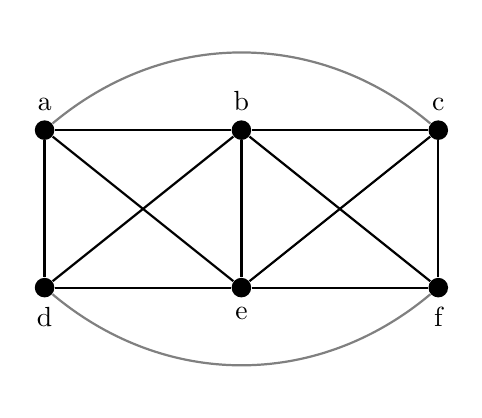
\begin{tikzpicture}[
          vtx/.style={circle, fill=black, inner sep=2.5pt, minimum size=5pt},
          edge/.style={draw, thick, black},
          curved/.style={draw, thick, gray}
        ]

        % Define node coordinates and labels
        \node[vtx, label=above:a] (a) at (0, 2) {};
        \node[vtx, label=above:b] (b) at (2.5, 2) {};
        \node[vtx, label=above:c] (c) at (5, 2) {};
        \node[vtx, label=below:d] (d) at (0, 0) {};
        \node[vtx, label=below:e] (e) at (2.5, 0) {};
        \node[vtx, label=below:f] (f) at (5, 0) {};

        % Draw all the straight edges
        \path[edge]
        (a) edge (b)
        (b) edge (c)
        (d) edge (e)
        (e) edge (f)
        (a) edge (d)
        (b) edge (e)
        (c) edge (f)
        (a) edge (e)
        (b) edge (d)
        (b) edge (f)
        (c) edge (e);

        % Draw the curved outer edges
        \path[curved]
        (a) edge [bend left=40] (c)
        (d) edge [bend right=40] (f);

      \end{tikzpicture}
    \end{center}

    Notice that the subgraph of $G$ obtained by removing edges $[f,
    e]$ and $[f, b]$ is homeomorphic to $K_5.$ If we start from the
    vertices $a, b, c, d, e$ labelled on $K_5,$ and then introduce an
    elementary subdivision described by  $[c, d] \to \{[c, f], [f,
    d]\},$ we get the graph:

    \begin{center}
      \begin{tikzpicture}[
          vtx/.style={circle, fill=black, inner sep=2.5pt, minimum size=5pt},
          edge/.style={draw, thick, black}
        ]
        % Define node coordinates (regular pentagon, radius 2.5)
        % Vertices at angles 90, 162, 234, 306, 378(=18) degrees
        \node[vtx, label=above:a]       (a) at (90:2.5)  {};
        \node[vtx, label=above left:b]  (b) at (162:2.5) {};
        \node[vtx, label=below left:c]  (c) at (234:2.5) {};
        \node[vtx, label=below right:d] (d) at (306:2.5) {};
        \node[vtx, label=above right:e] (e) at (18:2.5)  {};
        \node[vtx, label=above right:f, fill=red] (f) at (0, {2.5*sin(234)});

        % Draw all edges (complete graph K_5)
        \path[edge]
        (a) edge (b)
        (a) edge (c)
        (a) edge (d)
        (a) edge (e)
        (b) edge (c)
        (b) edge (d)
        (b) edge (e)
        (c) edge (f)
        (c) edge (e)
        (d) edge (e)
        (f) edge (d);
      \end{tikzpicture}
    \end{center}
    which is homeomorphic to $K_5$ and a subgraph of $G.$ By
    Kuratowski's theorem, $G$ cannot be planar.

    \newpage

  \item We proceed via induction.
    \paragraph{Base Case.} When $n = 3,$ the chromatic polynomial of
    cycle $C_3$ is $$\lambda(\lambda - 1)(\lambda - 2) = \lambda^3 -
    3\lambda^2 + 2\lambda = (\lambda - 1)^3 + (-1)^3(\lambda -1),$$
    meaning $P(C_n, \lambda) = (\lambda - 1)^n + (-1)^n (\lambda -
    1)$ when $n = 3.$

    \paragraph{Inductive Step.} Assume that the chromatic polynomial
    of a cycle $C_k$ is described by
    \begin{align*}
      P(C_k, \lambda) = (\lambda-1)^k  +(-1)^k (\lambda - 1).
    \end{align*}
    Consider a cycle of length $k + 1,$ $C_{k+1}.$ Using deletion
    contraction recursion, we know
    \begin{align*}
      P(C_{k+1}, \lambda) = P(P_{k+1}, \lambda) - P(C_{k}, \lambda).
    \end{align*}
    For a path $P_{k+1},$ the leading vertex has $\lambda$
    possibilities, and the remaining $k$ vertices have $\lambda - 1$
    options, meaning
    \begin{align*}
      P(P_{k+1}, \lambda)  = \lambda(\lambda - 1)^k.
    \end{align*}
    Thus, by our inductive hypothesis we have
    \begin{align*}
      P(C_{k+1}, \lambda) &= \lambda(\lambda - 1)^k -  [(\lambda-1)^k
      + (-1)^k(\lambda - 1)] \\
      &= (\lambda - 1)^{k+1} + (-1)^{k+1}(\lambda - 1),
    \end{align*}
    as required.

    Therefore, by mathematical induction $P(C_n, \lambda) =
    (\lambda-1)^n + (-1)^n(\lambda - 1)$ for all integers $n \geq 3.$

    \newpage

  \item
    \begin{enumerate}
      \item We use deletion-contraction on the edge $[1, 3]$:
        \begin{itemize}
          \item \textbf{Deletion yielding graph $G_d$.} Yields a
            cycle $C_4$ labeled $2, \ldots, 4$ alongside a vertex $1$
            connected to vertex $2.$ The $\lambda$-coloring of the
            cycle can be achieved in $(\lambda -1)^4 + (\lambda - 1)$
            ways by Q2, and then the vertex $1$ has $\lambda - 1$
            possible ways to be colored. Thus, $$P(G_d, \lambda ) =
            (\lambda-1)^5 + (\lambda - 1)^2.$$

          \item \textbf{Contraction yielding graph $G_c.$} After
            contraction, $G_c \cong C_4,$ meaning the chromatic polynomial is
            \begin{align*}
              P(G_c, \lambda) = (\lambda-1)^4 + (\lambda - 1).
            \end{align*}
        \end{itemize}

        By deletion-contraction, our chromatic polynomial is therefore
        \begin{align*}
          P(G, \lambda) = (\lambda - 1)^5 - (\lambda - 1)^4 +
          (\lambda - 1)^2 - (\lambda - 1).
        \end{align*}

      \item We split the graph $G$ into two subgraphs, one isomorphic
        to $C_3$ and another isomorphic to $C_4,$ with their
        intersection being isomorphic to $K_2$ (the edge $[2, 3]$).
        Therefore, we know
        \begin{align*}
          P(G, \lambda) = \dfrac{P(C_3, \lambda) \cdot P(C_4,
          \lambda)}{P(K_2, \lambda)} &= \dfrac{[(\lambda -1)^3 -
            (\lambda - 1)][(\lambda - 1)^4 + (\lambda -
          1)]}{\lambda(\lambda - 1)} \\
          &= \dfrac{[(\lambda - 1)^2 -1 ][(\lambda -1)^4 + (\lambda -
        1))]}{\lambda} \\
        &= (\lambda - 2)[(\lambda -1)^4 + (\lambda - 1)] \\
        &= (\lambda -1)^5 + (\lambda - 1)^2 - (\lambda -1)^4 - (\lambda - 1)
      \end{align*}

    \item Expanding the chromatic polymomial, we get
      \begin{align*}
        P(G, \lambda) = \lambda^5 - 6\lambda^4 + 14\lambda^3 - 15
        \lambda^2 + 6\lambda
      \end{align*}

      Since $P(G, 2) = 32 - 96 + 112 - 60 + 12 = 0,$ and $P(G, 3) =
      243 - 486 + 378 - 135 + 18 = 18 > 0,$ $\chi(G) = 3.$
  \end{enumerate}
\end{enumerate}
\end{document}
